\documentclass[../../main]{subfiles}

\renewcommand\thesection{\arabic{section}}


\begin{document}

\section{Thermal Control} \label{sec:}

The thermal control system mainly consists of four parts, the \emph{core
block}, \emph{dedicated coolers}, \emph{intake panels} and \emph{exhaust
pipes}. At the heart of \emph{core block} lies a \emph{peltier} module. Along
with this, the core block has three chambers, seven panels, and three fans. We
will see details about these in the following sections. But before that let's
get familiarized with the peltier module.

\subsection{Heating / Cooling Element}

The \emph{thermals} of the Incubator can be controlled using a \emph{peltier} module, which is
\emph{semi-conductor} based \emph{heat engine}. The COP\footnote{Coefficient of Performance.} is
much less than a typical \emph{compressor} based \emph{heat pumps} and is \emph{variable} depending
on the current passing through it. But the compactness of the \emph{peltier} cooler makes it preferable
to this design. One another disadvantage to this type of cooling is that it requires a proper \emph{exhaust}
system. Peltier coolers only decrease the temperature of their \emph{cold} side to relative to their
\emph{hot} side\footnote{The \emph{cold} side will be $30 - 40^\circ$C colder than its \emph{hot} side.}.
The \emph{peltier} module is thin, that means the \emph{hot} and \emph{cold} are closer. So it is
\emph{crucial} to properly pull away the heat from its \emph{cold} side as fast as possible.

We will be using \emph{TEC12703} peltier, with the specifications as:

\begin{itemize}
    \item \textbf{Operating voltage.:} $3\si{V}$ to $15\si{V}$.
    \item \textbf{I Max.:} $3\si{A}$.
    \item \textbf{Power:} $30\si{W}$.
\end{itemize}

Figures \ref{fig:peltierImage} and \ref{fig:peltierHSImage} shows the peltier and the heatsink
used.

\begin{center}
    \begin{tabularx} {\textwidth} {
            >{\centering \arraybackslash}X
            >{\centering \arraybackslash}X
            >{\centering \arraybackslash}X
        }


        \toprule

        \emph{TEC12703} module. & Heat sink & Relay cubes \\ \midrule

        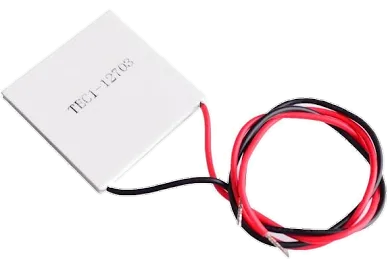
\includegraphics[
            width = 0.25\textwidth,
        ] {pics/peltier.png}

        &
        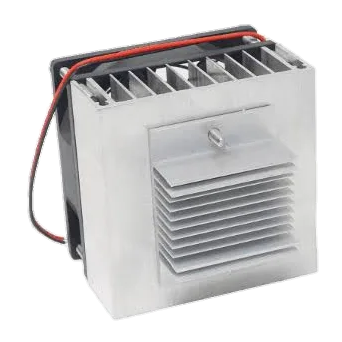
\includegraphics[
            width = 0.25\textwidth,
        ] {pics/peltier_hs.png}

        &

        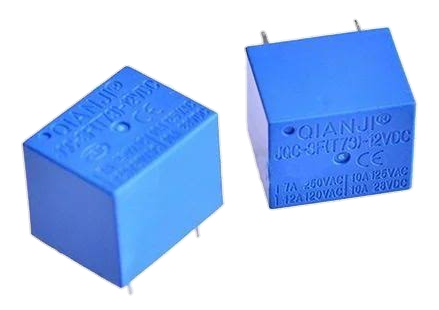
\includegraphics[
            width = 0.25\textwidth,
        ] {pics/sugar_cube.png}

        \\

        \captionof{figure}[\emph{TEC12703} module.]{}
        \label{fig:peltierImage}
        &
        \captionof{figure}[Heat sink for \emph{TEC12703} peltier module.]{}
        \label{fig:peltierHSImage}
        &
        \captionof{figure}[Relay sugar cubes.]{}

        \vspace{-2.0cm}

        \\

        \bottomrule

    \end{tabularx}

    \captionof {table} {Peltier module and components required for its use.}

\end{center}

\alertNote{
    Peltier module is also controlled via a relay, since it can pull almost $2.7A$ when
    connected to a 12V power supply.
}

\end{document}
